%!TEX root = ../thesis.tex

\chapter{Результати дослідження}
\label{chap:research_results} 

На початку доcлідження було виявлено, що бібілотеки створюються, як правило, трьома способами:
\begin{enumerate}
	\item реалізуються на мовах C/C++ і використовується там же;
	\item реалізуються тою мовою, де їх будуть використовувати (до прикладу, крейт \href{https://docs.rs/crypto-bigint/latest/crypto_bigint/}{crypto-bigint} у Rust);
	\item спочатку реалізуються як із пункту 1, а потім пишеться певна обгортка над операціями/типами задля легкості використання.
\end{enumerate}

Спробуємо провести аналіз деяких із представників цих бібліотек.


\section{С/С++ бібліотеки}
Спочатку наведемо короткий опис із бібіліотек, що можна було взяти до аналізу прямо із завдання лабораторної роботи. Потрібно одразу попередити, що поки для нас C/C++ дається важко для написання своїх прикладів(. Наведемо доступні бібліотеки.

\begin{itemize}
	\item Pari/GP -- спеціалізована комп'ютерна алгебраїчна система, що у більшості використовується науковцями для різних областей від топології чи числового аналізу до фізики. Як зрозуміли, то GP у ній є такою собі спеціалізованою скриптовою мовою, а PARI, що є безпосередньо \href{https://pari.math.u-bordeaux.fr/pub/pari/manuals/2.7.6/libpari.pdf}{libpari} бібліотекою написаною на С.
		
	\begin{figure}[!h]
    		\centering
    		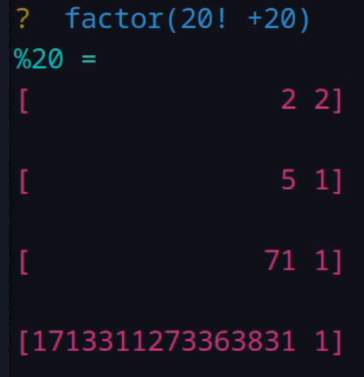
\includegraphics[scale = 0.30]{IMAGES/Rust/pari_gp}
    		\caption{Приклад факторизації числа $20! + 20$ на мові GP.}
    		\label{fig:}
	\end{figure}

	
	\item GNU GMP -- безкоштовна бібліотека для арифметики довільної точності, яка працює над цілими числами зі знаком, раціональними числами та числами з плаваючою комою. Тут немає жодних практичних обмежень точності, окрім тих, що передбачають доступну пам’ять у машині, на якій працює GMP. GMP  має багатий набір функцій, і функції мають звичайний інтерфейс.
	
	\begin{figure}[!h]
    		\centering
    		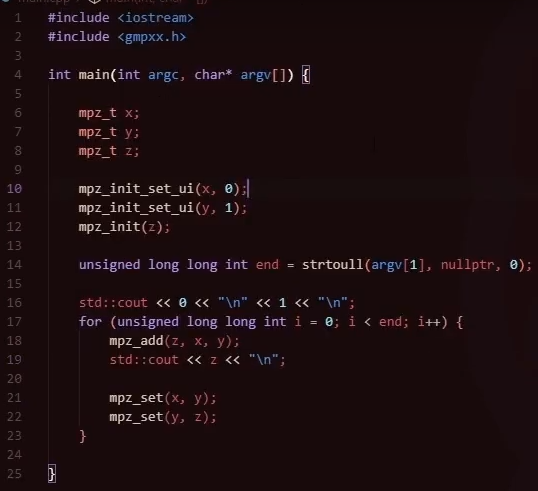
\includegraphics[scale = 0.47]{IMAGES/Rust/gnu_gmp}
    		\caption{Приклад виводу у циклі підсумованих великих чисел із використанням  типів GNU GMP бібліотеки.}
    		\label{fig:}
	\end{figure}
\end{itemize}


\section{Rust}

У світі сучасної розробки програмного забезпечення мова програмування Rust завоювала своє місце, завдяки вражаючій комбінації ефективності та безпеки. Ця мова програмування може використовуватися для розробки від операціних систем до аналізу даних. Тож розгляньмо ключові бібліотеки Rust, що можуть бути використані для великих обчислень.

\subsection{Обгортки над С/С++}

\begin{itemize}
	\item \href{https://crates.io/crates/rug}{Rug} -- обгортка над C/C++, що написана на Rust, надає цілі числа та числа з плаваючою комою з довільною точністю та округленням разом із операціями над ними. Саме ця бібліотека реалізовує високорівневий інтерфейс над бібліотеками GNU:
	\begin{itemize}
		\item GMP (для цілих чисел та раціональних чисел),
		\item MPFR (для чисел із плаваючою точкою),
		\item MPC (для комплексних чисел).
	\end{itemize}
		
	Надалі наведу трохи скрішотів та пояснень до коду для цілочисельного типу. 
    Почнемо із піднесення до степеня.
	\begin{figure}[!h]
    		\centering
    		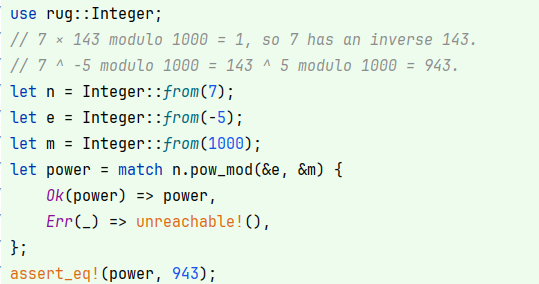
\includegraphics[scale = 0.45]{IMAGES/Rust/pow_mod_rug}
    		\caption{Приклад використання піднесення до степеня за модулем.}
    		\label{fig:pow_mod_rug}
	\end{figure}
	
	\begin{figure}[!h]
    		\centering
    		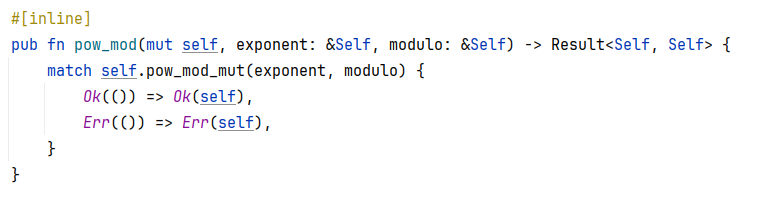
\includegraphics[scale = 0.45]{IMAGES/Rust/pow_mod_rug_code1}
    		\caption{Код який використовує функція \ref{fig:pow_mod_rug}.}
    		\label{fig:pow_mod_rug_code1}
	\end{figure}
	
	\begin{figure}[!h]
    		\centering
    		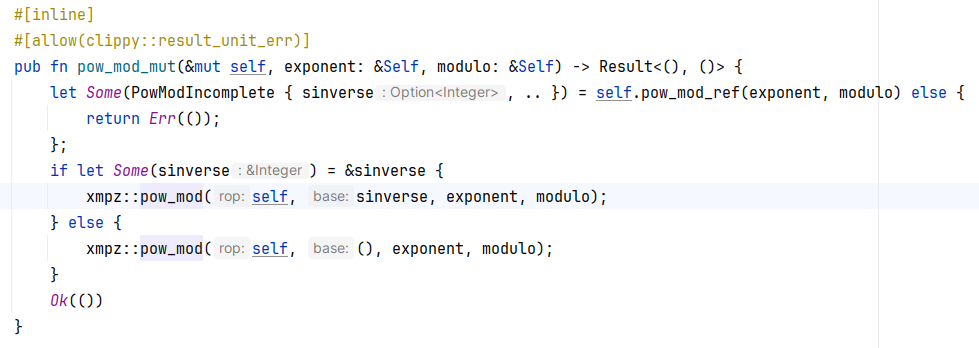
\includegraphics[scale = 0.45]{IMAGES/Rust/pow_mod_rug_code2}
    		\caption{Далі функція \ref{fig:pow_mod_rug_code1} переходить сюди.}
    		\label{fig:pow_mod_rug_code2}
	\end{figure}	
	
	\begin{figure}[!h]
    		\centering
    		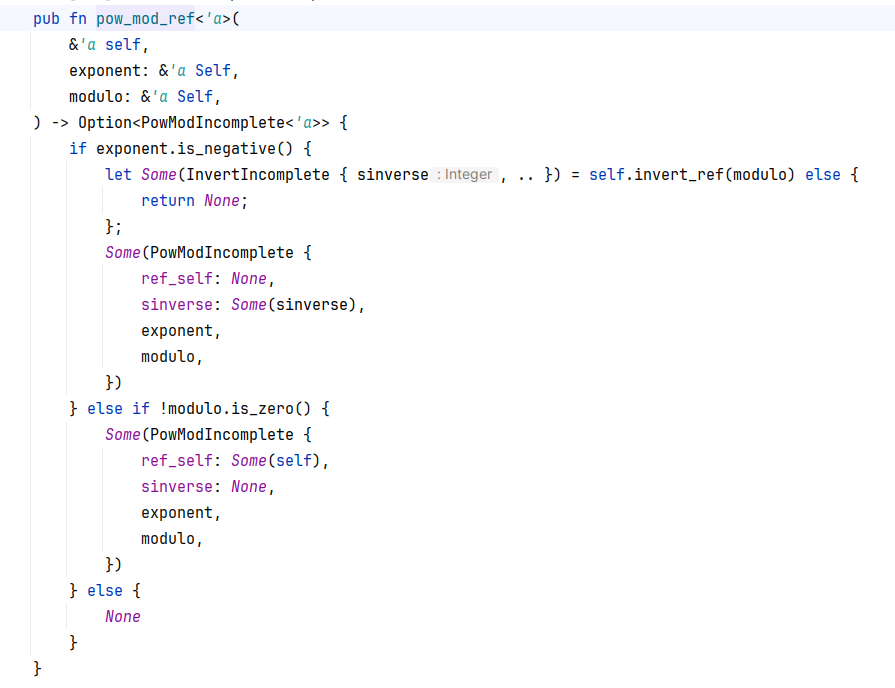
\includegraphics[scale = 0.45]{IMAGES/Rust/pow_mod_rug_safe}
    		\caption{За умови збереженого значення переходимо у цю функцію із \ref{fig:pow_mod_rug_code2}.}
    		\label{fig:pow_mod_rug_safe}
	\end{figure}	
	
	\begin{figure}[!h]
    		\centering
    		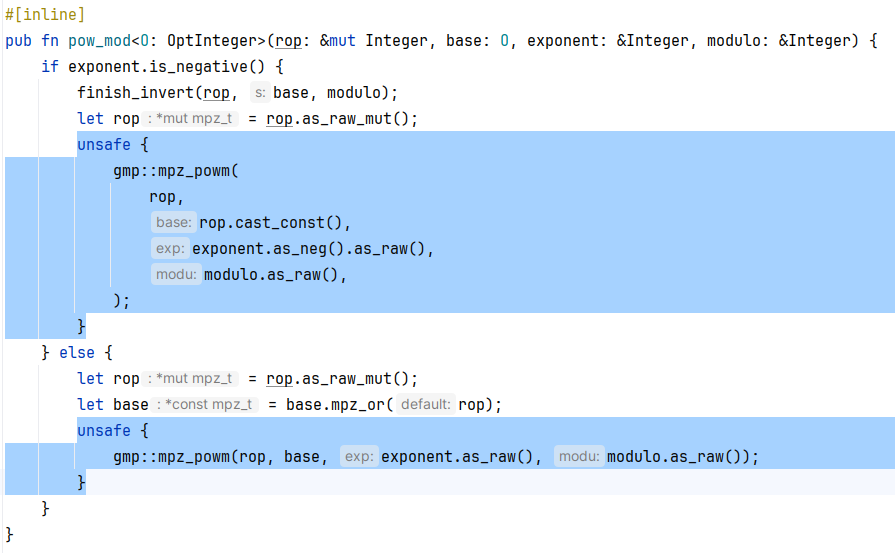
\includegraphics[scale = 0.45]{IMAGES/Rust/pow_mod_rug_unsafe}
    		\caption{Задля обчислення числа заново, переходимо сюди із \ref{fig:pow_mod_rug_code2}.}
    		\label{fig:pow_mod_rug_unsafe}
	\end{figure}
	
	Тепер пояснимо код піднесення до степеня. Перший скріншот \ref{fig:pow_mod_rug} є прикладом до використання. Потім як передемо по коду, передемо до скріншоту \ref{fig:pow_mod_rug_code1} -- це є відправною точкою. Далі від неї переходимо у функцію \ref{fig:pow_mod_rug_code2}. Вона має у собі розвилку, де \ref{fig:pow_mod_rug_safe} переходить і повертає збережені значення як такі є, а \ref{fig:pow_mod_rug_unsafe} спускається до виклику функції із C. Усе це можливо завдяки FFI(Foreign Funciton Interface), що є певним механізмом, де програма написана на одній мові програмування може використовувати бібліотеки/сервіси написані на іншій мові програмування. У Rust FFI забезпечує абстракцію та сумісність без витрат, що зводиться до швидкості виконання коду на C. 
 
    Наведемо ще один приклад функції. Цього разу будемо викликати пошук оберненого.
	
	\begin{figure}[!h]
    		\centering
    		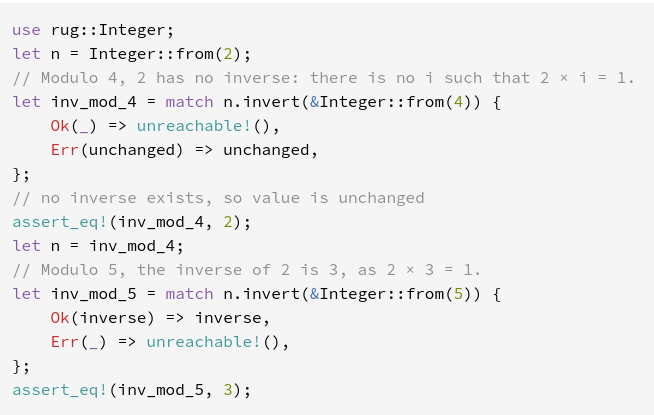
\includegraphics[scale = 0.45]{IMAGES/Rust/inverse_rug_example}
    		\caption{Приклад використання функції invert().}
    		\label{fig:inverse_rug_example}
	\end{figure}
	
	\begin{figure}[!h]
    		\centering
    		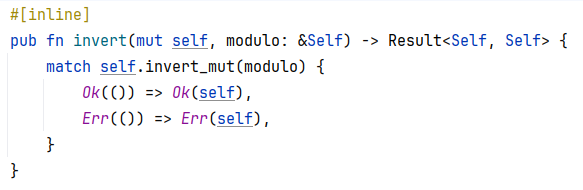
\includegraphics[scale = 0.45]{IMAGES/Rust/inverse_rug_code1}
    		\caption{Сама функція inverse().}
    		\label{fig:inverse_rug_code1}
	\end{figure}
	
	\begin{figure}[!h]
    		\centering
    		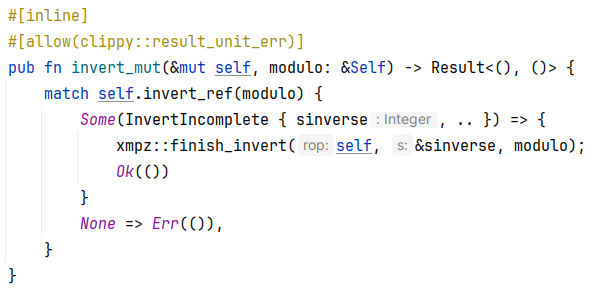
\includegraphics[scale = 0.45]{IMAGES/Rust/inverse_rug_code2}
    		\caption{Переходимо сюди із \ref{fig:inverse_rug_code1}.}
    		\label{fig:inverse_rug_code2}
	\end{figure}
	
	\begin{figure}[!h]
    		\centering
    		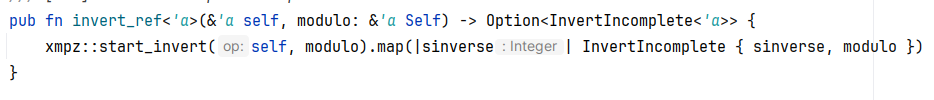
\includegraphics[scale = 0.45]{IMAGES/Rust/inverse_rug_code3}
    		\caption{Остання функція для переходу із \ref{fig:inverse_rug_code2}.}
    		\label{fig:inverse_rug_code3}
	\end{figure}
	
	Перший скрішнот \ref{fig:inverse_rug_example} показує приклад використання оберненого за модулем, де за будь-яких умов повертається число. Тільки у негативному випадку всеодно отримаємо число для якого повинно було б бути обчислено обернений елемент. Прейшовши до \ref{fig:inverse_rug_code1}, можна побачити, що все зводиться до виклику іншої функції \ref{fig:inverse_rug_code2}, яка навпаки, замість повернення нового елементу, мутує даний на вхід об'єкт. Далі перейшовши до \ref{fig:inverse_rug_code3}, можна побачити, що знову ж усе зводиться до обгорнутих функцій від C/C++ бібліотеки. 
	
\end{itemize}

\subsection{Нативні бібліотеки}

\begin{itemize}

\item Одна із бібліотек, про яку б хотіли розповісти -- \href{https://crates.io/crates/crypto-bigint}{crypto-bigint}, що реалізована знову на Rust. Її особливістю є те, що вона підтримується спільнотою, що робить криптологічні крейти для Rust. Також можна додати, що вона використовує у собі багато макросів, що рекурсивно генерують код для певних значень.

	Сама бібліотека реалізована ефективно, зокрема використовує такий собі підхід константних значень до яких може бути реалізовано код за потреби макросами. 
	Ось, наприклад, є приклад макросу \ref{fig:crypto-bigint-macros_mod}, який у свою чергу може бути розписаний у \ref{fig:crypto-bigint-macros_mod2} 

	\begin{figure}[!h]
	    \centering
    		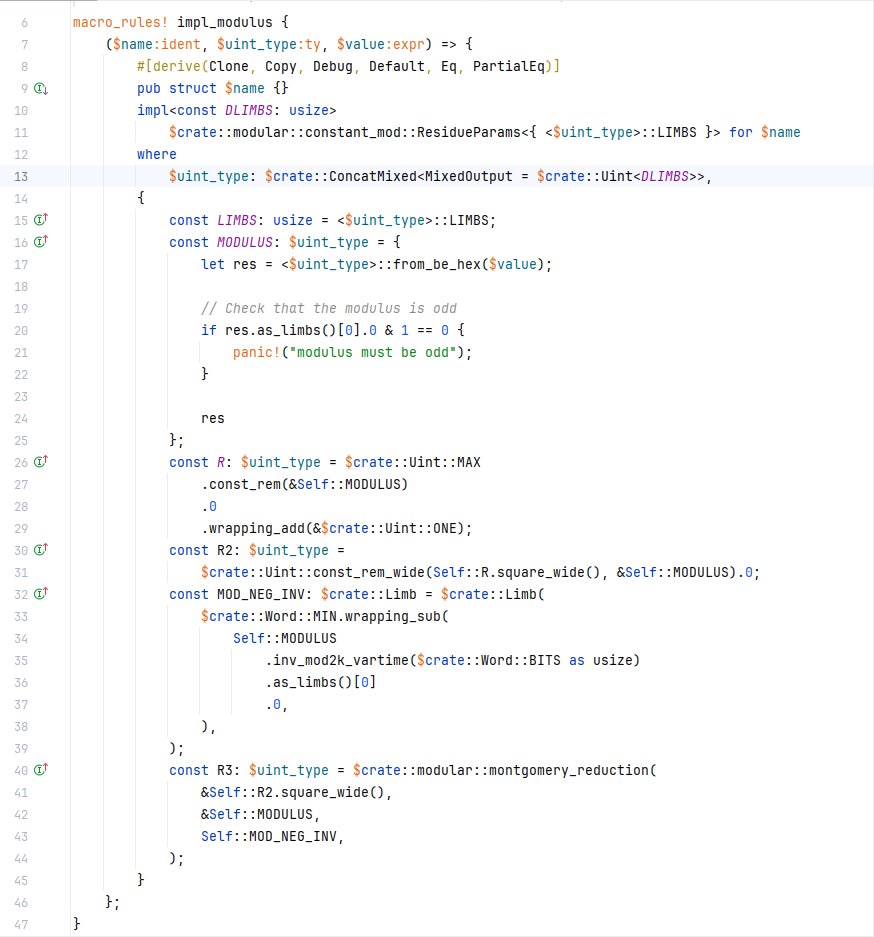
\includegraphics[scale = 0.45]{IMAGES/Rust/crypto-bigint-macros_mod}
	    \caption{Приклад синтаксису макросу у crypto-bigint.}
    		\label{fig:crypto-bigint-macros_mod}
	\end{figure}

	\begin{figure}[!h]
	    \centering
    		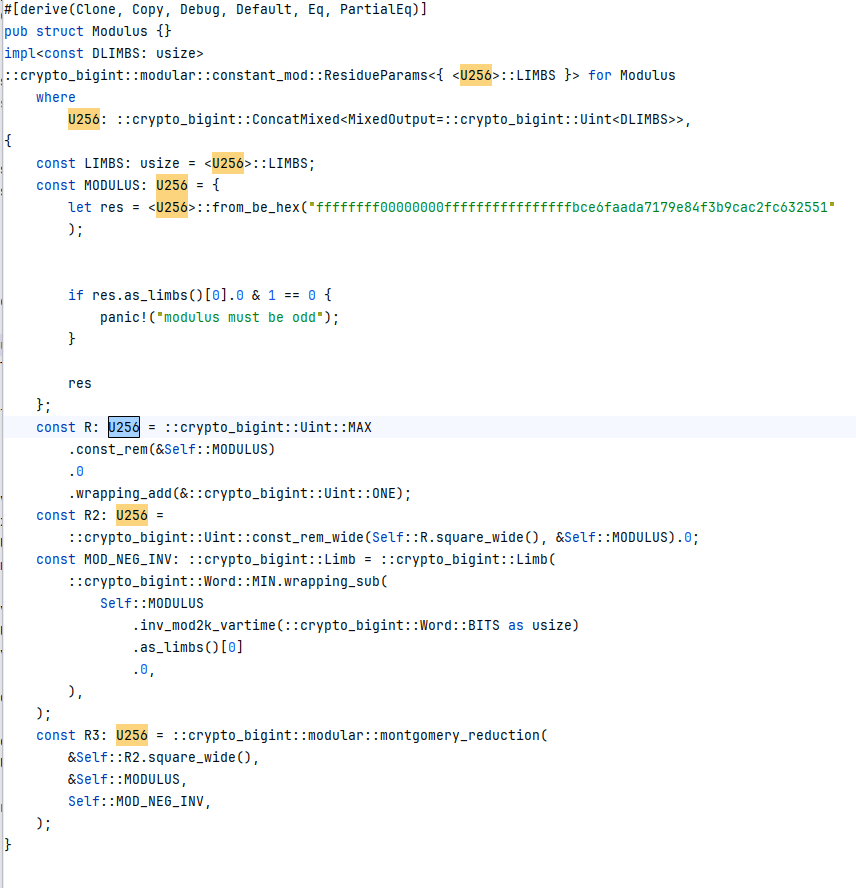
\includegraphics[scale = 0.45]{IMAGES/Rust/crypto-bigint-macros_mod2}
	    \caption{Приклад розширення макросу для типу U256.}
    		\label{fig:crypto-bigint-macros_mod2}
	\end{figure}

	Як можна побачити, тут була застосована основна родзинка Rust. 
	У тому, що можна написати код, який буде сам себе генерурвати для нових подібних типів або буде скорочувати роботу розробнику.

\item Також розповім про останню, просто досить популярну бібліотеку, яку, зокрема, використовував для лабораторних робіт. Це є \href{https://crates.io/crates/num-bigint}{num-bigint} простою ефективною бібліотекою, де реалізовані знакові та беззнакові числа, використання різних баз для створення великих чисел (32, 64, 128 бітні числа). Зокрема у ній реалізовані ефективні алгортими множення (Карацуби та Toom-3) та на додачу редукцію Монтгомері разом із іншими оптимізованими операціями. Також додам, що приклад використання цієї біліотеки є у папці \textbf{./rust}. Там наведена реалізація 3 лабораторної роботи із асиметричної криптографії.
\end{itemize}
